A continuación se muestra el diagrama en bloques de hardware y los delimitadores de las distintas secciones, siendo estas:
\begin{itemize}
\item Potencia.
%\item Cargador.
\item Sensado.
\end{itemize}

\begin{figure}[H]
	\centering
	%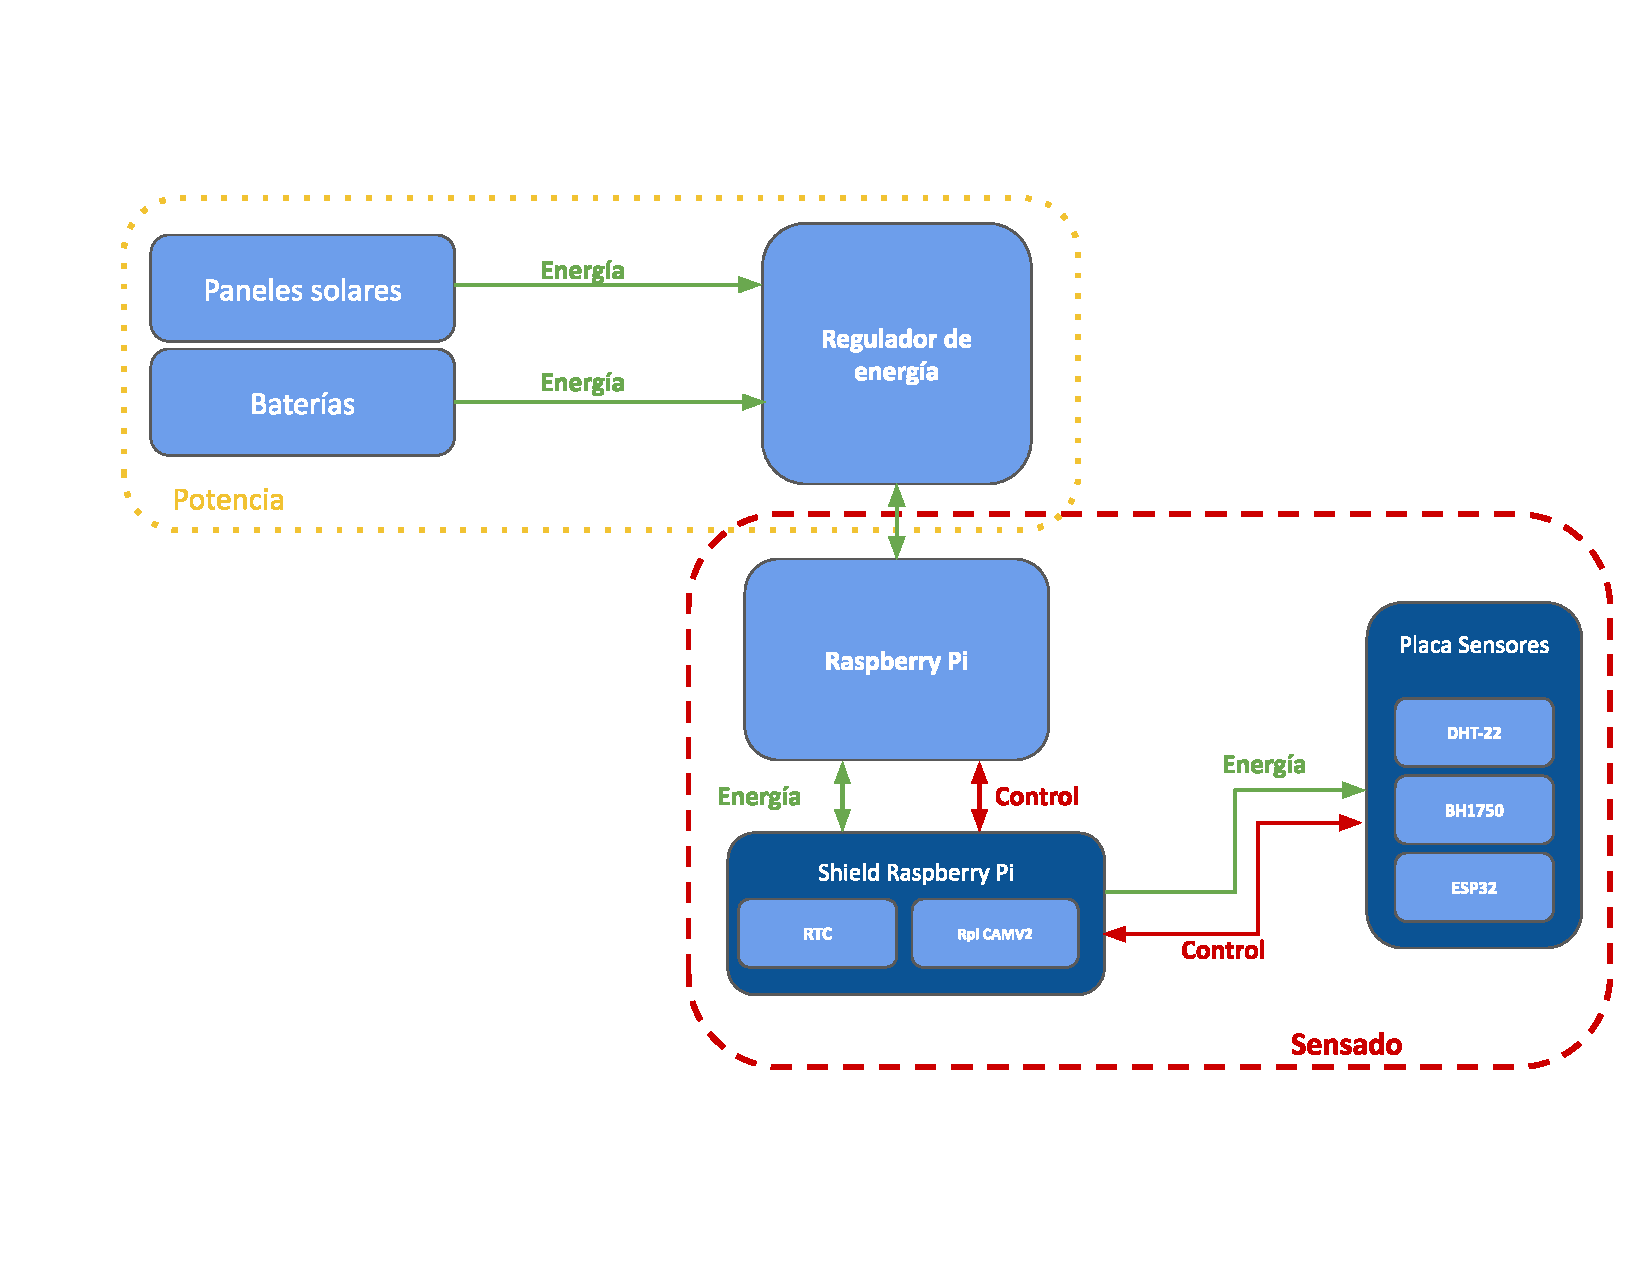
\includegraphics[width=0.7\linewidth]{ImagenesIngenieria de Detalle/DiagramaHardwareMarcado}
	\includegraphics[width=0.7\textwidth, page=7]{ImagenesIngenieria de Detalle/FlowChart.pdf}		
	\caption{Diagrama en bloques del sistema de hardware.}
	\label{fig:diagrama_hardware}
\end{figure}

La etapa de potencia es el conjunto de elementos necesarios para proveer de energía a toda la electrónica del proyecto, es decir a aquellos componentes y elementos que se encuentran en el nido.

%El cargador es la etapa que se encarga, como su nombre indica realizar al carga inalámbrica de la UBM.

Por otro lado, la de sensado es aquella que se encarga de la medición de las variables físicas y de su correcto almacenamiento, teniendo en cuenta que esto implica un conocimiento preciso de la hora.